\section{Шаги по времени}\label{sec:time}

Возьмём простейшее движение, которое поворачивает: $y'=i\,y$; его точное решение идёт по
окружности. Один шаг $s$ должен повернуть $y$ на $s$. Три классических одношаговых правила
помещают точку в три разных места, и это снова три пути.

\begin{itemize}
  \item \textbf{Явный метод Эйлера}, $y\mapsto(1+is)\,y$, шагает вдоль касательной. Его
    модуль равен $\sqrt{1+s^2}>1$, поэтому он уходит с окружности наружу и на каждом шаге набирает энергию.
  \item \textbf{Неявный метод Эйлера}, $y\mapsto y/(1-is)$, имеет модуль $1/\sqrt{1+s^2}<1$. Он падает
    внутрь окружности и на каждом шаге теряет энергию.
  \item \textbf{Метод Кранка~--- Николсон}, $y\mapsto\frac{1+is/2}{1-is/2}\,y$, есть отображение Кэли с
    $\tau=s/2$. Он остаётся точно на окружности, но поворачивает на $\varphi=2\arctan(s/2)$. Шаг
    $s$ играет роль внешнего пути $T$, а фактически совершённый поворот~--- дуга.
    Фазовое запаздывание равно $s-\varphi=\tfrac{1}{12}s^3+O(s^5)$~--- та же $1/12$, что и в $T-A$ в
    предложении~\ref{prop:lengths}.
\end{itemize}
На рис.~\ref{fig:time} показаны три правила на протяжении одного полного оборота.

\begin{figure}[t]\centering
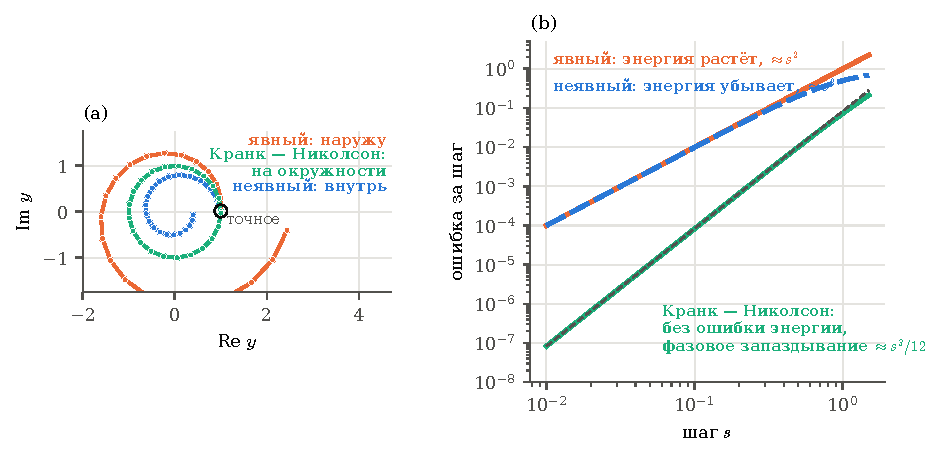
\includegraphics[width=\linewidth]{figures/fig_time.pdf}
\caption{Шаги по времени для $y'=iy$. \textbf{(a)} Двадцать один шаг величины $s=0.3$ (один полный
оборот, $t\approx2\pi$) из $y=1$. Явный метод Эйлера (оранжевый) раскручивается по спирали наружу, неявный метод Эйлера (синий)
закручивается внутрь, а метод Кранка~--- Николсон (зелёный) остаётся на окружности; пустой кружок отмечает точный
конец. \textbf{(b)} Ошибка за шаг: методы Эйлера набирают или теряют энергию порядка $s^2$
(кривые явного и неявного методов совпадают в главном порядке), тогда как метод Кранка~--- Николсон не делает
ошибки в энергии и отстаёт по фазе на $s-2\arctan(s/2)\approx s^3/12$ (штриховая линия).}
\label{fig:time}
\end{figure}

\paragraph{Три спирали, одна из них золотая.} Каждый шаг явного метода Эйлера умножает
модуль на $\sqrt{1+s^2}$ и поворачивает на $\arctan s$, так что отношение роста к повороту никогда
не меняется. Поэтому каждая получаемая им точка лежит точно на логарифмической (равноугольной)
спирали, \emph{spira mirabilis} Якоба Бернулли,
\[
r=e^{b\theta},\qquad b(s)=\frac{\ln(1+s^2)}{2\arctan s}.
\]
Неявный метод Эйлера лежит на зеркальной спирали $r=e^{-b\theta}$, её близнеце с тем же наклоном, а
метод Кранка~--- Николсон~--- член семейства с нулевым наклоном: окружность между ними. При шаге с
рис.~\ref{fig:time}(a), $s=0.3$, внешняя спираль растёт в $1.2614$ раза за каждую четверть
оборота, при наклоне $8.41^\circ$. Золотая спираль~--- это член семейства, растущий в
$\varphi=(1+\sqrt5)/2$ раз за каждую четверть оборота, $b=2\ln\varphi/\pi\approx0.3063$, при наклоне
$17.03^\circ$. Спираль Фибоначчи из четвертей окружностей, вписанных в квадраты, приближает её, потому что
отношения соседних чисел Фибоначчи стремятся к $\varphi$. Поскольку $b(s)$ возрастает по $s$,
существует ровно один шаг, при котором явный метод Эйлера точно вычерчивает золотую спираль:
$s^\ast\approx0.6515$, или $33.08^\circ$ поворота за шаг. Золотой случай принадлежит этому единственному
шагу. Это член семейства, которое рисует метод, а не свойство самого метода.

Для общего линейного потока $y'=-Gy$ множитель Кранка~--- Николсон
$r(z)=(1-z/2)/(1+z/2)$ удовлетворяет $|r(z)|\le1$ ровно тогда, когда $\operatorname{Re}z\ge0$. Его
поведение на ненормальной матрице $G$ определяется числовым образом $W(G)$. По теореме
Крузе~--- Паленсии \cite{cp}, $\|r(hG)^k\|\le(1+\sqrt2)\sup_{z\in W(G)}|r(hz)|^k$. На группе
Ли отображение Кэли сохраняет каждое обновление точно на $SU(2)$ \cite{iserles}.

\begin{plain}
Моделировать что-то вращающееся~--- значит продвигать его вперёд понемногу, шаг за шагом. Самый простой
шаг уходит вдоль боковой линии и сползает наружу, набирая энергию, которой у него быть не должно.
Обратный вариант сползает внутрь и теряет энергию. Шаг Кэли, отрезок обхода, остаётся
точно на окружности и лишь немного отстаёт~--- на ту же одну двенадцатую, что отделяет
обход от истинного пути. Если нарисовать много шагов, сползание наружу вычерчивает логарифмическую
спираль, из того же семейства, что и золотая спираль, а при одном размере шага она в точности золотая.
Сползание внутрь~--- её зеркальный близнец, а шаг Кэли~--- окружность между ними. Поэтому
он оказался естественным правилом для моделирования потока на сетке, и сопутствующая статья теперь им
пользуется: восемь шагов Кэли следуют за потоком так же точно, как много маленьких явных шагов. Собственные
часы движка по-прежнему шагают вдоль истинной кривой (раздел~\ref{sec:gigi}).
\end{plain}

\section{Близнецы, обратная сторона и Бертран}\label{sec:twins}

\paragraph{У каждого промаха есть близнец с другой стороны.} Оценка Снеллиуса~--- Гюйгенса
$(2C+T)/3$ даёт избыток относительно дуги. Другая оценка Снеллиуса даёт недостачу:
\[
L=\frac{6\sin(\theta/2)}{2+\cos(\theta/2)},\qquad
\theta-L=\tfrac{1}{2880}\theta^5+O(\theta^7),\qquad L<\theta<\frac{2C+T}{3}.
\]
Два промаха равны $\theta^5/320$ сверху и $\theta^5/2880$ снизу, девять к одному. Значит, близнецов
можно снова смешать, $\tfrac{1}{10}\bigl(9L+\tfrac{2C+T}{3}\bigr)=\theta+O(\theta^7)$, и
смесь оставляет меньшую пару близнецов. Каждое сокращение порождает следующее.

\paragraph{Близнец с обратной стороны.} Хорда не знает, в какую сторону шёл поворот.
Повороты $\theta$ и $2\pi-\theta$ имеют одну и ту же хорду. Внешний путь знает: его
отрезок касательной меняет знак, $\tan\bigl((2\pi-\theta)/2\bigr)=-\tan(\theta/2)$, потому что
вершина, где встречаются касательные, переходит на другую сторону окружности.

\paragraph{Где находится вершина.} Прямая хорды лежит на расстоянии $p=\cos(\theta/2)$
от центра, а вершина~--- на расстоянии $1/p$ (полюс и поляра). Положение вершины
определяет режим.
\begin{itemize}
  \item \emph{Вершина вне окружности} ($0<p<1$): всё вещественно.
  \item \emph{Прямая хорды проходит через центр} ($p=0$, полуоборот): касательные
    параллельны, и вершина находится в бесконечности. За этой точкой вершина возвращается с обратной стороны;
    это близнец с обратной стороны. Переход через центр переключает на близнеца, и всё остаётся вещественным.
  \item \emph{Вершина внутри окружности} ($p>1$; прямая хорды не пересекает окружность):
    две концевые точки становятся комплексно сопряжённой парой, и поворот становится мнимым,
    $\theta=i\varphi$. Тогда $C=2i\sinh(\varphi/2)$, отрезок касательной равен $i\tanh(\varphi/2)$, и
    $S=\cosh^2(\varphi/2)>1$. Тождество $S+d^2=1$ сохраняется, с мнимым $d=i\sinh(\varphi/2)$.
    Окружность превратилась в гиперболу, а поворот~--- в буст. Именно переход через границу окружности
    делает числа невещественными.
\end{itemize}

\paragraph{Парадокс Бертрана.} Бертран спросил, какова вероятность того, что «случайная хорда»
длиннее стороны вписанного правильного треугольника \cite{bertrand}. Ответ
зависит от того, как выбирается хорда, и каждый классический способ делает равномерно распределённой
одну из величин этой статьи:
\begin{center}\small
\begin{tabular}{lll}\toprule
Способ выбора хорды & Равномерная величина & Вероятность \\ \midrule
две случайные концевые точки & дуга $\theta$ & $1/3$ \\
случайное расстояние вдоль радиуса & $\sqrt S=\cos(\theta/2)$ & $1/2$ \\
случайная середина & сходство $S$ & $1/4$ \\
\bottomrule\end{tabular}
\end{center}
Хорда больше $\sqrt3$ ровно тогда, когда $\theta>2\pi/3$, $\cos(\theta/2)<1/2$ и $S<1/4$, так что
три ответа получаются сразу. Моделирование с двумя миллионами хорд на каждый способ даёт
$0.3333$, $0.5004$ и $0.2498$. Внешний путь не даёт четвёртого ответа такого рода: его отрезок уходит в
бесконечность при полуобороте, поэтому его нельзя распределить равномерно. Джейнс утверждал, что инвариантность
относительно сдвигов и изменения масштаба окружности выделяет способ с радиусом \cite{jaynes}.

Группа поворотов всё же даёт четвёртый ответ, потому что у неё есть собственный честный способ
выбрать поворот случайно~--- мера Хаара, которая не оставляет нам никакого выбора. Для равномерно
распределённого случайного единичного кватерниона геодезический угол $a$ имеет плотность $(2/\pi)\sin^2a$ на $[0,\pi]$, поэтому
сходство $S=\cos^2(a/2)$ подчиняется закону полукруга $(8/\pi)\sqrt{S(1-S)}$ на $[0,1]$. Событие
Бертрана~--- это $S<1/4$, и его вероятность равна
\[
\tfrac13-\tfrac{\sqrt3}{4\pi}\approx0.19550,
\]
что не совпадает ни с одним из трёх классических ответов. Моделирование четырёх миллионов случайных поворотов даёт
$0.19545$ (\path{scripts/haar_sameness.py} в репозитории GIGI).

\begin{plain}
У каждой оценки, которая промахивается в одну сторону, есть близнец, промахивающийся в другую, и смешивание
близнецов убирает промах, оставляя пару поменьше. У хорды тоже есть поворот-близнец: если пойти длинным
путём вокруг, хорда будет та же, но обход это замечает, потому что его вершина перескакивает на
другую сторону. Где стоит эта вершина, решает всё. Снаружи окружности всё вещественно.
Через центр~--- вы переходите к близнецу. Внутри окружности числа становятся мнимыми,
окружность становится гиперболой, и всё равно $S+d^2=1$ выполняется. Знаменитый парадокс Бертрана~--- это
тот же вопрос в другом обличье: «случайная хорда» ничего не значит, пока вы не скажете, какую из этих
величин вы распределяете равномерно: дугу, квадратный корень из сходства или само
сходство.
\end{plain}
